\begin{figure}
  \centering
  
  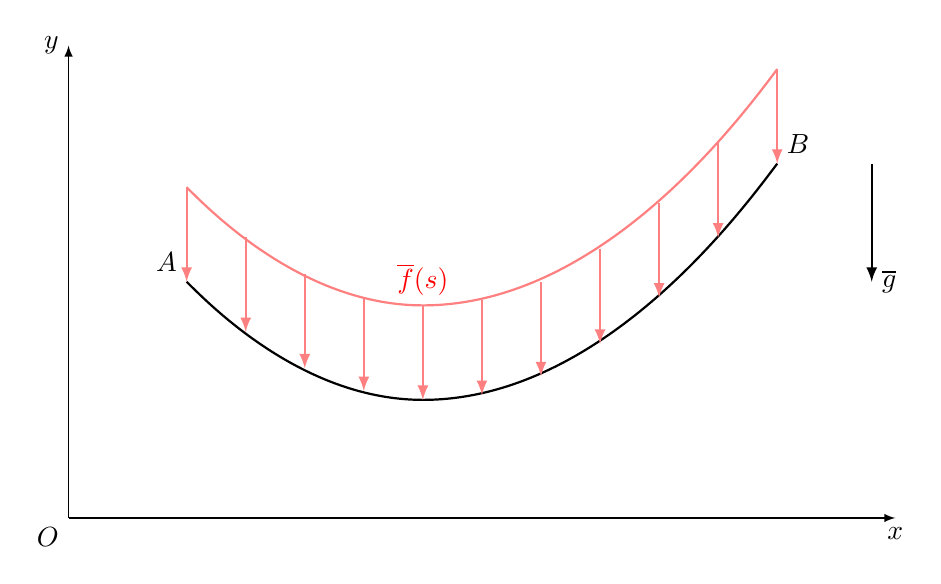
\begin{tikzpicture}[scale = 1.5]
   
     \draw [-latex] (0,0) -- (7,0) node [below] {$x$};
     \draw [-latex] (0,0) -- (0,4) node [left] {$y$};
     \node at (0,0) [below left] {$O$};
 
     \draw [thick] (1,2) parabola  bend (3,1) (6,3);
     \node at (1,2) [above left] {$A$};
     \node at (6,3) [above right] {$B$};

     \foreach \x in {1,1.5,...,6}
     \draw [red!50, latex-, thick] (\x, \x*\x*7/30 - \x*43/30 +16/5) --+ (0,.8);

     \begin{scope}[shift = {(0,.8)}]
      \draw [red!50, thick] (1,2) parabola  bend (3,1) (6,3);
      \node at (3,1) [color = red, above] {$\overline{f}(s)$};
     \end{scope}
 
   \draw [-latex, thick] (6.8,3)--(6.8,2) node [right] {$\overline{g}$};

  \end{tikzpicture}
  
  \caption{Problema della catenari omogenea}
  \label{fig:problema_catenaria_omogenea}
  
  
  
 \end{figure}
